\begin{figure}
\centering
\begin{subfigure}{\textwidth}
  \centering
  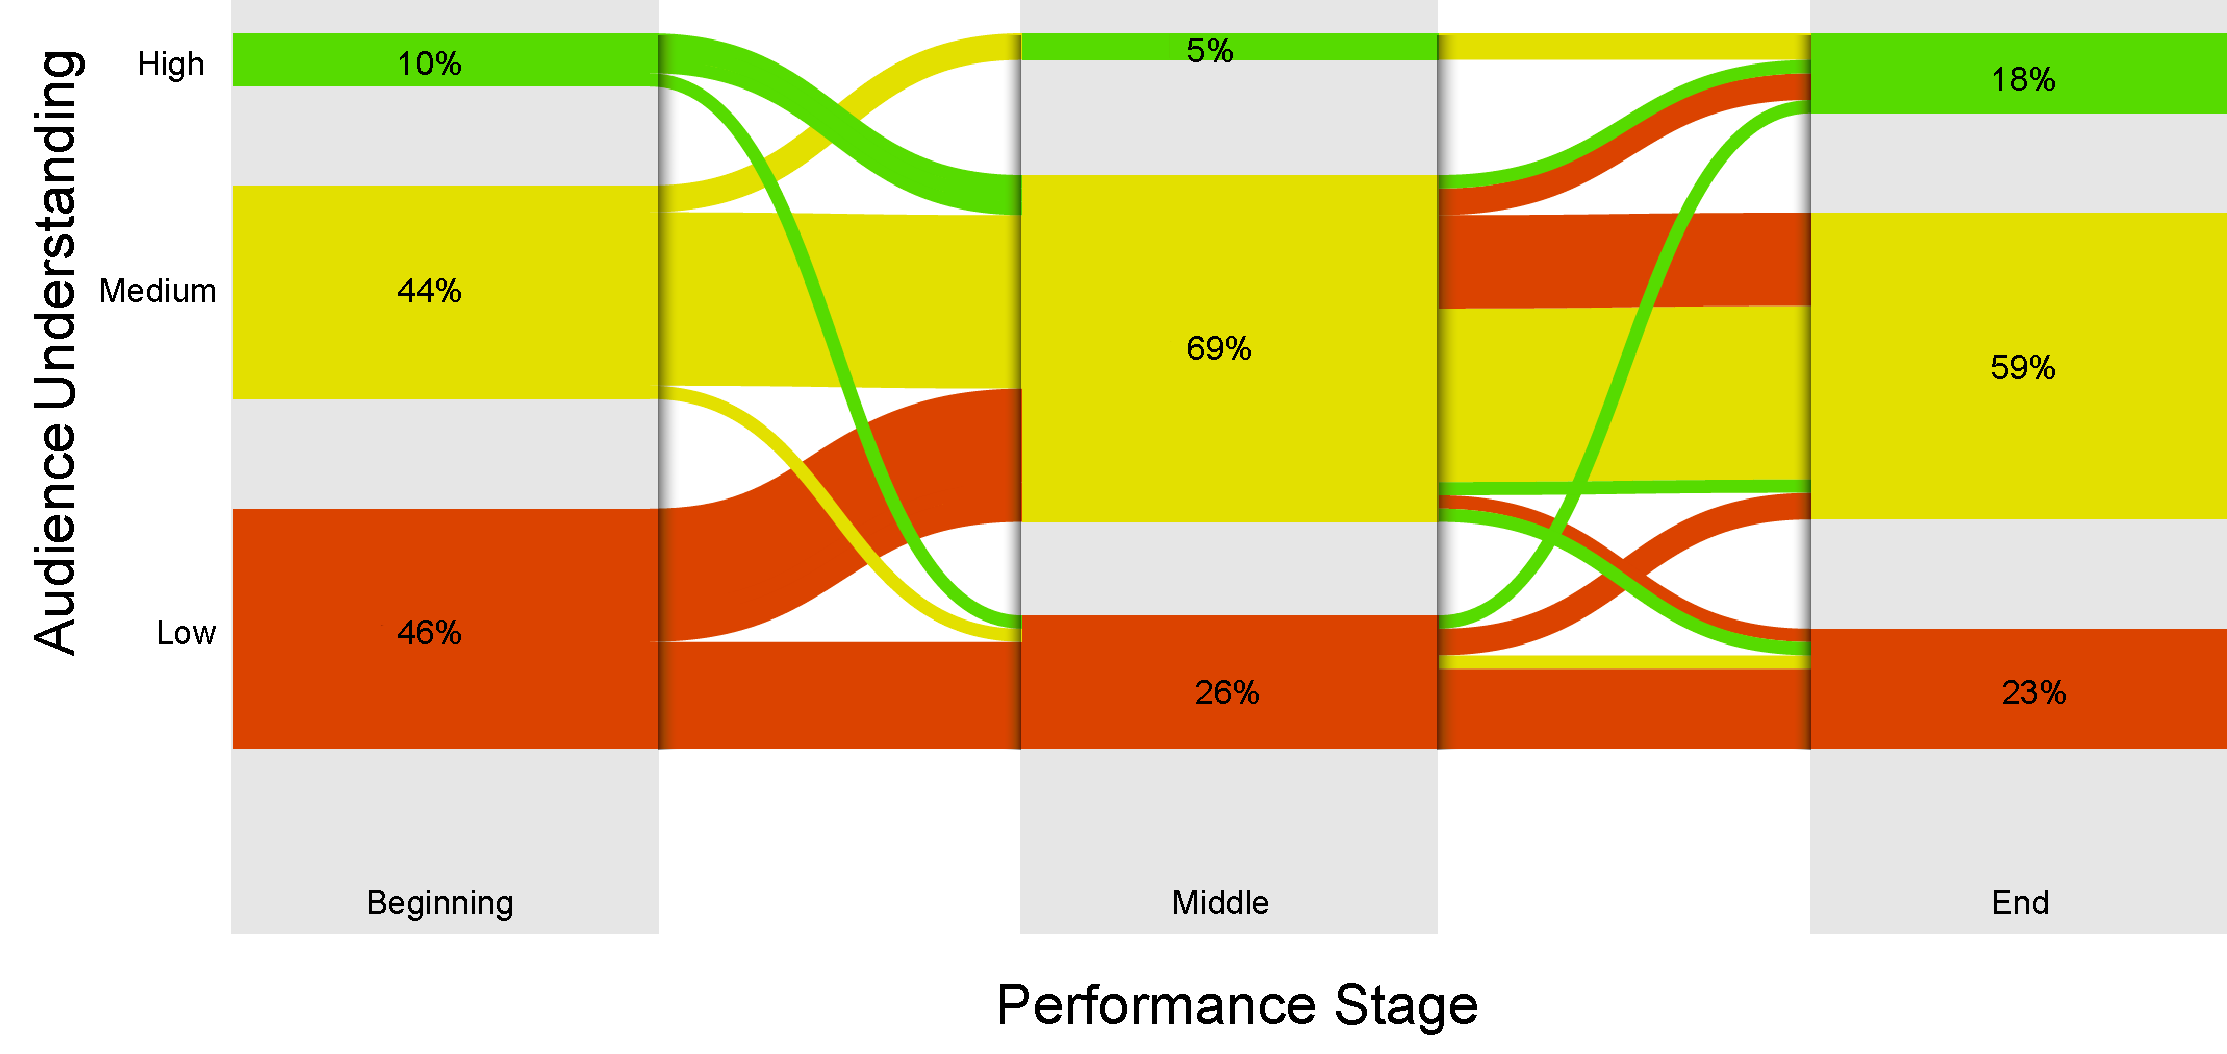
\includegraphics[width=\columnwidth,page=1]{../images/graphs/condition-dimension.pdf}
  \caption[Didactic condition understanding detailed survey results]{Audience reported understanding level for the \textbf{didactic} condition.}
  \label{fig:didactic-understanding}
\end{subfigure}\\
\begin{subfigure}{\textwidth}
  \centering
  \includegraphics[width=\columnwidth,page=2]{../images/graphs/condition-dimension.pdf}
  \caption[Aesthetic condition understanding detailed survey results]{Audience-reported understanding level for the \textbf{aesthetic} condition.}
  \label{fig:aesthetic-understanding}
\end{subfigure}

\caption[User study understanding survey responses]{Audience reported understanding during the beginning, middle and end of the performance for the didactic and aesthetic visualisation conditions. Line width at each stage indicates proportion of the audience reporting high, medium or low understanding, and line colour connecting each section of the performance is determined by the understanding level at the \emph{beginning} of the performance.}
\label{fig:user-study-condition-understanding}
\end{figure}